\chapter{Methods}
\label{cha:methods}

\redtxt{Pendent: parlar sobre theil sen ???}

This chapter centers on the implementation of the models defined in Chapter \ref{cha:model} and the optimization method outlined in Section \ref{sec:introduction_model_optimization}.
Section \ref{sec:methods_model-implementation} focuses on the implementation of the models in a \CC{} program, including a class hierarchy diagram, several important algorithms, various methods used to avoid floating point error and the different distributions of $\pi$ (see Section \ref{sec:model_math_second-model}) that were implemented.
Section \ref{sec:methods_optimization} deals with the optimization algorithm, how it changes for the static or dynamic cases and several optimizations that allow for faster runtime and more precise results.
On Section \ref{sec:methods_parallelization} the approach taken to parallelization is outlined and justified.
Section \ref{sec:methods_verification} deals with the verification of the code.
Finally, Section \ref{sec:methods_num-prec-probs} explains the main challenges related to numerical precision while Section \ref{sec:methods_other-probs} covers other problems related to the implementation.

\section{Model implementation}
\label{sec:methods_model-implementation}

This section covers the implementation of the two models seen in Chapter \ref{cha:model}.
It starts with a class hierarchy diagram of the organization of the static and dynamic versions of the two models.
Following this, the algorithm used to randomly generate a random bipartite graph (given a vertex probability or given the number of edges) is outlined.
Following this, the various ``tricks'' used in order to minimize the floating point error, specially in the dynamic version of the model are explained.
To close this section, details on the various distributions of $\pi$ that were implemented are given.

\subsubsection{Class hierarchy diagram}

The diagram in Figure \ref{fig:class-diagram} shows the classes implementing the bipartite graph models (see Chapter \ref{cha:model}).

\begin{figure}
  \centering
  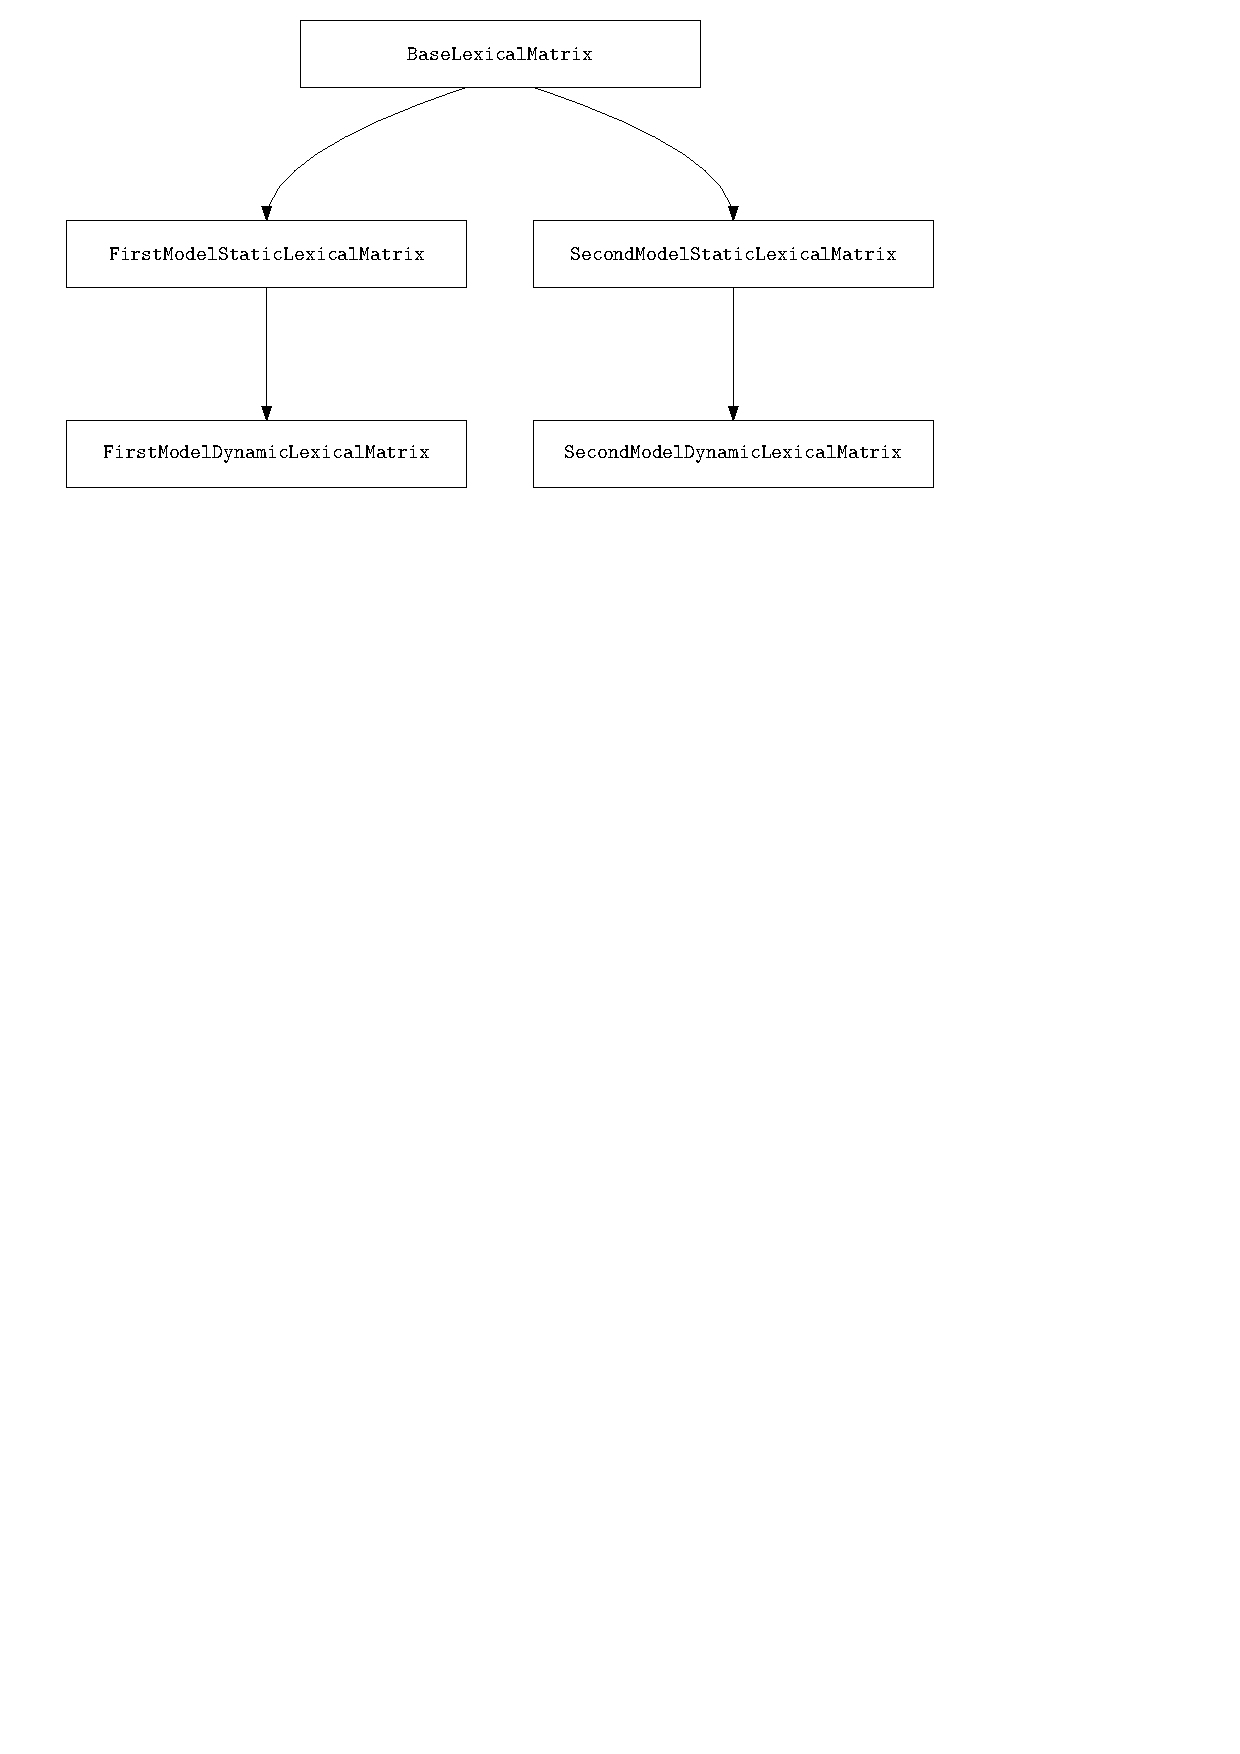
\includegraphics[width=\textwidth]{class_diagram}
  \caption{Diagram showing the hierarchy of the classes implementing the two models in their dynamic and static variants in the \CC{} program.}
  \label{fig:class-diagram}
\end{figure}

\subsubsection{Random graph generation}

This section outlines the algorithm implemented to generate a random Erdos-Renyi bipartite graph \cite{Erdos1960} in pseudocode.
The graph can be generated by specifying either the probability of edge creation ($G_{n,m,p}$) as seen in Algorithm \ref{alg:gnmp} or the total number of edges ($G_{n,m,e}$) as in Algorithm \ref{alg:gnme}.
Note that all Algorithm \ref{alg:gnmp} actually does is compute a value of $e$ then call Algorithm \ref{alg:gnme}.

\begin{algorithm}
  \caption{$G_{n,m,p}$ algorithm to generate a random \nbym{} graph given probability of edge $p$.} \label{alg:gnmp}
\begin{algorithmic}[1]
  \Procedure{$G$}{$n,m,p$}
    \State $e \gets$ \Call{binom}{$n \cdot m$, $p$}
    \State \Return \Call{G}{$n,m,e$}
  \EndProcedure
\end{algorithmic}
\end{algorithm}

\begin{algorithm}
  \caption{$G_{n,m,e}$ algorithm to generate a random \nbym{} graph given the number of edges $e$.} \label{alg:gnme}
  \begin{algorithmic}[1]
    \Procedure{$G$}{$n,m,e$}
      \If{disconnected meanings disallowed}
        \For{each $r_j$ such that $1 \leq j \leq m$}
          \State $s_i \gets$ \Call{uniform}{$s_1$, $s_n$}
          \State \Call{add edge}{$s_i, r_j$}
          \State $e \gets e - 1$
        \EndFor
      \EndIf
      \While{$e > 0$}
        \State $s_i \gets$ \Call{uniform}{$s_1$, $s_n$}
        \State $r_j \gets$ \Call{uniform}{$r_1$, $r_n$}
        \State \Call{add edge}{$s_i, r_j$}
        \State $e \gets e - 1$
      \EndWhile
    \EndProcedure  
  \end{algorithmic}
\end{algorithm}

\subsubsection{Dealing with floating point error}

One of the major challenges (see Section \ref{sec:methods_num-prec-probs} has been dealing with floating point error.
Two major ``tricks'' have been used in order to minimize this loss of precision as much as possible.

\paragraph{The Accumulator class}
Whenever possible, specially in the static calculations, additions have been done through an accumulator class.
This class maintains two variables, \texttt{total} and \texttt{current}.
When a value is added, it is added to the \texttt{current} variable.
If the \texttt{current} variable is greater than \texttt{total}, it is added to \texttt{total} and reset to 0.
This is an inexpensive and effective way to minimize the loss of precision from a common occurrence during static calculation, the addition of a smaller value into a greater one.

\paragraph{Static recalculation}
During the optimization process, whenever a new minimum is reached, a static recalculation is forced.
In this way, one of the major source of floating point error from the dynamic version is removed.
The dynamic equations (see Section \ref{sec:model_math}) consist of many additions and subtractions.
These additions and subtractions are a major contributor to the accumulation of floating point error.
Since finding a new minimum is not common, this does not affect the run time of the optimization process.

\paragraph{Save and restore}
Most steps of the optimization process will not improve the cost function (see Section \ref{sec:methods_optimization}).
Instead of undoing the step and recalculating all the parameters of the model, the parameters are saved before performing the step, and they are restored when the step needs to be reverted.
This strategy reduces the amount of additions and subtractions to be done when the recalculation of parameters is dynamic, thus reducing the amount of floating point error.

\subsubsection{Distribution of $\pi$}

The second model (see Section \ref{sec:model_math_second-model}) is based on a vector of length $m$ of \emph{a priori} probabilities $\pi$.
Uniform, geometric, power law and broken stick probability distributions have been implemented in order to give values to the elements of this vector.

\paragraph{Uniform distribution} The uniform distribution simply assigns the probability $1/m$ to every element in the vector.

\paragraph{Geometric distribution} Assigns a right truncated geometric distribution with parameter $p$ to the elements of $\pi$, following
\begin{equation*}
  (1-p)^{x-1} \frac{p}{1 - (1-p)^m}.
\end{equation*}
This formula can be easily derived from the more general formula for a truncated discrete probability distribution
\begin{equation*}
  P(X=x | a < x \leq b) = p(X=x) / (P(X=b) - P(X=a)).
\end{equation*}

\paragraph{Power law distribution} Assigns a right truncated power law distribution with parameter $\alpha$ to the elements of $\pi$.
It follows
\begin{equation*}
  x^{-\alpha} \sum_{i=1}^m i^{-\alpha}
\end{equation*}

\paragraph{Broken stick distribution} A broken stick distribution corresponds to the distribution of the sizes of the pieces of a stick that is broken by a point along its length randomly a number $m-1$ of times.
This distribution corresponds to the expected value of the lengths of the pieces of a stick of total length 1.
The formula and its derivation is given in \cite{Smart1976a} (Equation 1).

\section{Optimization}
\label{sec:methods_optimization}

The optimization algorithm follows the Markov Chain Monte Carlo method at zero temperature.
The model is initialized in some way (depending on parameters), and on each iteration a number of random mutations (adding or removing an edge on the underlying bipartite graph) are effectuated.
The cost function is evaluated with a parameter $\lambda$.
If it is found to have improved, the model is recalculated statically (to avoid floating point error, see Section \ref{sec:methods_model-implementation}).
If it is found to not have improved, the changes are reverted.
The optimization stops after a number of failures to improve the cost function.
The optimization stops early if the lower bound of the cost function is reached (See Equation \eqref{eq:lower-bound-Omega}).

The parameter $\lambda$ is given as a parameter.
It controls the weight of the two forces that contribute to the cost function.
See Section \ref{sec:introduction_model_optimization}.

The number of mutations done on each step depends on the parameters and may be either constant or follow a binomial distribution.
In the case of a binomial distribution, it is possible that zero mutations may be effectuated.
In this case, nothing is done and the step is considered to not have improved the cost function.

The number of failures to improve the cost function needed to stop iterating depends on parameters.
Two possible values are calculated from parameters of the model:
\begin{itemize}
\item \textbf{weak}:
  Enough steps are performed such that it is likely that all edges have been visited once.
  This follows the Coupon Collector's Problem \cite{Mitzenmacher2017}, and the formula for the number of attempts is
  \begin{equation*}
    \lfloor nm \log nm \rfloor
  \end{equation*}
\item \textbf{strong}:
  Enough steps are performed such that it is likely that every possible pair of edges has been visited once.
  This also follows the Coupon Collector's Problem,
  \begin{equation*}
    \left\lfloor {nm \choose 2} \log {nm \choose 2} \right\rfloor
  \end{equation*}
\end{itemize}

\section{Parallelization}
\label{sec:methods_parallelization}

During the initial phases of the design of the software, it was considered to add parallelization in order to speed up calculations.
Parallelization would add overhead and complexity to an already complex codebase in exchange for sharing the computation between the machine's processors.

A typical task for the program is the computation of a range of values of $\lambda$ (see Section \ref{sec:methods_optimization}) and to calculate several samples for each $\lambda$.
This layout lends itself well to multiprocessing, without the program implementing any sort of parallelization scheme.

The user is expected to divide the load his or herself, for instance by generating many separate configuration files (or using a script to do so) and using a tool such as one of the many implementations of \texttt{parallel} or a computing cluster's workload manager.
In this way, the operating system handles the parallelization complexity and the software's complexity and overhead is reduced.
This also makes verification much easier.

\section{Verification}
\label{sec:methods_verification}

Verification is a vital part of any software development process.
In this case, verification involves ensuring that both static and dynamic versions of the model are correctly implemented.
Dynamic versions are specially complex and so need to be tested thoroughly.

The test routines implemented verify that the models give ``sane'' results by checking extreme cases (see Sections ).
In addition, the invariants of the entropies (also in Sections ) are verified after every mutation and the program is aborted if they ever do not hold.
A test also checks the invariants exhaustively for every possible combination of connected and disconnected edges for very small graphs ($n=m=4$).

Other functionality less related with the implementation of the model is also tested.
\begin{itemize}
\item The save/restore functionality described in Section \ref{sec:methods_model-implementation} for dealing with floating point error.
\item Quickly testing whether the matrix has disconnected meanings (configuration parameter disallows disconnected meanings).
\end{itemize}

The last test is running the program for relatively small values of $n$ and $m$ and all combinations of parameters, and exhaustively checking that both static and dynamic versions give identical output for the same seed.
This test is used to ensure the correctness of the dynamic version.

\section{Numerical precision problems}
\label{sec:methods_num-prec-probs}

Challenges and problems related to the numerical precision are given in this section.

In both the static and dynamic versions of the calculations, there are many additions or subtractions of floating point numbers.
These actions often involve a loss of precision due to the difference in magnitude of the values being operated.
Over many iterations, this loss of precision can become apparent and change the final result of the simulation.
See Section \ref{sec:methods_model-implementation} where an entire subsection is dedicated to dealing with numerical error.

The geometric distribution decreases in probability very quickly.
Because of this, erroneous values can be produced when the value of $\pi$ is too close to 0.
As outlined in Section \ref{sec:model_math_second-model}, the values of $\pi$ should never be zero.
This problem occurs in general whenever $\pi$ is too close to zero and the program automatically warns about it if the parameters will generate values of $\pi$ that are too small.
For this reason, the geometric distribution does not appear in Chapter \ref{cha:results}

\section{Other problems}
\label{sec:methods_other-probs}

Since the runtime of the dynamic versions often depends on the number of neighbors of the affected vertices (see Section \ref{sec:model_compute}), running calculations on complete or almost complete graphs takes a long time, as the advantages of the dynamic formulas are reduced significantly.
As a result of this, running the optimization with an initial complete graph can take an unacceptable amount of time when compared to other initial conditions.

The strong stop condition (Section \ref{sec:methods_optimization}) results far too many attempts to improve the cost function when $n=m$ is large (for $n=m=400$, the number of attempts is of the order of $10^{12}$).
For this reason, the strong stop condition is not used in Chapter \ref{cha:results}

%%% Local Variables:
%%% mode: latex
%%% TeX-master: "tfm"
%%% End:
